\section{Generalizing \sysname{}}
\label{sec:generic}

We now generalize the design of \sysname{} for any topology. First, we 
formalize the description of the tagging system. See Table~\ref{tab:symbols} for
notation.

Let $A_i$ represent a unique ingress port in the network, {\em i.e.,} switch
$A$'s $i^{th}$ ingress port.  We use a {\em tagged graph} $G(V,E)$ to uniquely
represent a tagging scheme.  Given a tagging scheme, the {\em tagged graph}
$G(V,E)$ is defined as: 

\begin{enumerate}
\item $G$ contains a node, $(A_i, x)$, {\em iff.} port $A_i$ may receive packets with tag $x$, and these packets must 
be lossless. $V$ is the set of all such nodes.

\item $G$ contains an edge $(A_i, x)\rightarrow(B_j, y)$ {\em iff.} switch $A$ and $B$ are 
connected, {\em and} switch $A$ may change a packet's tag from $x$ to $y$ before sending to $B$ (the case $x=y$ also counts).
$E$ is the set of all such edges.

\end{enumerate}

Given a tag $k$, we also define $\{G_k\}$, with vertices $V(G_k)$ and edges
$E(G_k)$: 
$$V(G_k) = \{(A_i, k) | \forall A, i\} $$
$$E(G_k) = \{v_0 \rightarrow v_1 | \forall v_0, v_1 \in V(G_k),  v_0 \rightarrow v_1 \in E(G)\} $$
Each tag $k$ is mapped to a unique lossless priority.  

Each node has a rule to match on a tag on an ingress port, and assign the packet
to corresponding lossless queue.  In addition, each edge corresponds to a switch
action of setting the tag for the next hop at the egress.

\begin{table}[t]
\small
\centering
\begin{tabular}{|c|c|}
\hline
Symbol & Description \\ \hline
$A_i$ & Switch $A$'s $i^{th}$ ingress port  \\ \hline
$(A_i, x)$ & A node in tagged graph \\ \hline
$(A_i, x)\rightarrow(B_j, y)$ & A tagged edge \\ \hline
$V$ & All tagged nodes  \\ \hline
$E$ & All tagged edges \\ \hline
$G(V, E)$ & Tagged graph \\ \hline
$G_k$ & Partition of $G(V,E)$ for priority $k$ \\ \hline
\end{tabular}
\caption{Notations in the formalized description.}
\label{tab:symbols}
		\vspace{-1em}
\end{table}

If a packet arrives at $A_i$ with tag $x$, and is destined for port $B_j$, and
there is no corresponding edge in $G(V,E)$, it means that the packet has
traversed on a path that is not expected to be lossless.  Such packets are
assigned a special tag, and all switches assign this tag to lossy
priority\footnote{This rule is always the last rule in the 
list, acting as a default safeguard that avoids unexpected buffer dependency.
See \S\ref{sec:implementation}.}.

In the rest of the section, we will describe how to generate the tagging graph
-- i.e. the tagging rules. But first, we prove that the tagging scheme described
by such a graph is deadlock free, as long as the graph meets two requirements.

\begin{enumerate} 

		\item  Any $G_k$ for $G$ {\em must not} have a cycle.  This is
				because each edge in $G_k$ is essentially a buffer dependency --
				whether $A_i$ can dequeue packets depending on whether $B_j$ has
				paused upstream. A cycle in $G_k$ means cyclic buffer
				dependency.  
		\item There must be no link going from
				$G_x$ to $G_y$ if $x>y$.  This means we enforce the order of
				$G_x$.
\end{enumerate}

These requirements are essentially generalization of the properties
discussed in \S\ref{subsec:specific_deadlock_free}. 

\begin{theorem}
Any tag system, defined by $G(V,E)$, that satisfies the above two requirements is deadlock-free.
\end{theorem}

\begin{proof}
We prove by contradiction. Suppose there exists a tag system,
whose $G(V,E)$ satisfies the above two requirements, but is not deadlock-free. This means
$G(V,E)$ has a cycle $v_0 \rightarrow v_1 \rightarrow ... \rightarrow v_0$. With certain 
traffic that covers all hops in the circle, the cycle turns into a CBD and can form deadlock.

\textbf{Case 1:} All the nodes in the cycle has the same tag $t$. According to
the first requirement, $G_t$ does {\em not} have a cycle. Contradicted.

\textbf{Case 2:} The nodes in the cycle have at least two different tags, $t_0$ and $t_1$.
Without loss of generality, we assume $t_0 < t_1$, and $v_i$ has tag $t_0$, $v_j$
has tag $t_1$. Because $v_i$ and $v_j$ belongs to a circle, there must exists 
a path going from $v_j$ to $v_i$. Since $t_0 < t_1$, there must exist a hop where
the tag decreases. However, according to the second requirement, such a hop cannot
exist. Contradicted.

Case 1 and Case 2 cover all possible scenarios. Thus, we conclude that there does not 
exist a $G(V,E)$ that satisfies the two requirements but is not deadlock-free.
\end{proof}

We now describe the algorithm to generate $G(V,E)$ for any given topology, and set of
paths that need to be lossless. 

\subsection{Generating $G(V,E)$} 
\begin{figure*}[t]
	\centering
	\subfloat[short for lof][Input topology and lossless routes.] {
		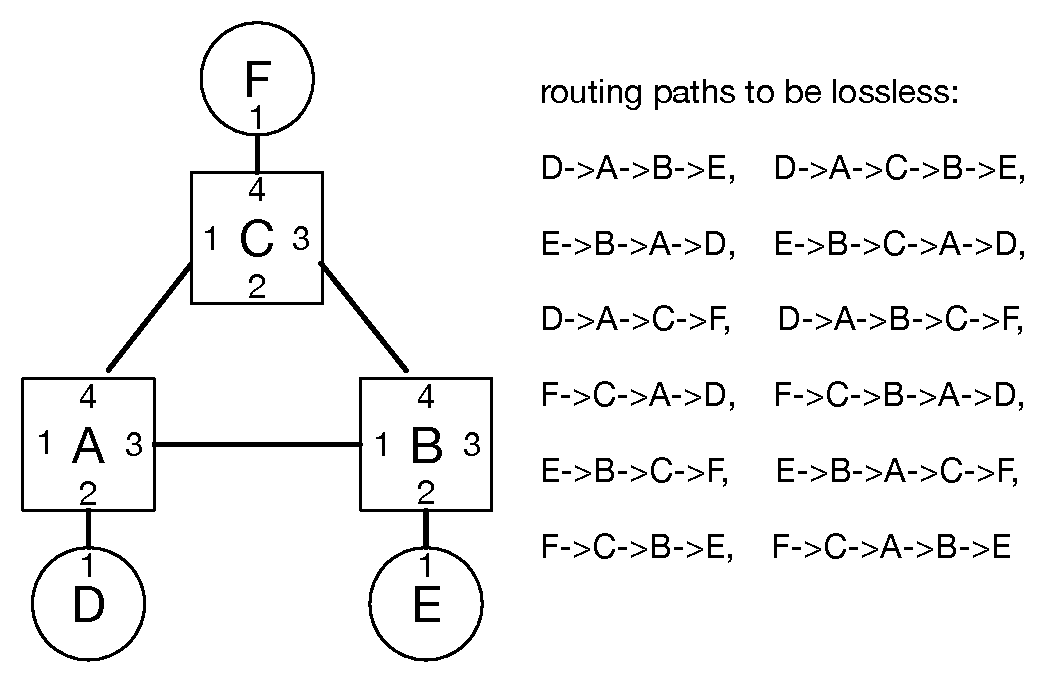
\includegraphics[width=0.6\textwidth] {figs/alo_walkthrough_a}
	}
	\subfloat[short for lof][Output tagged graph.]{
		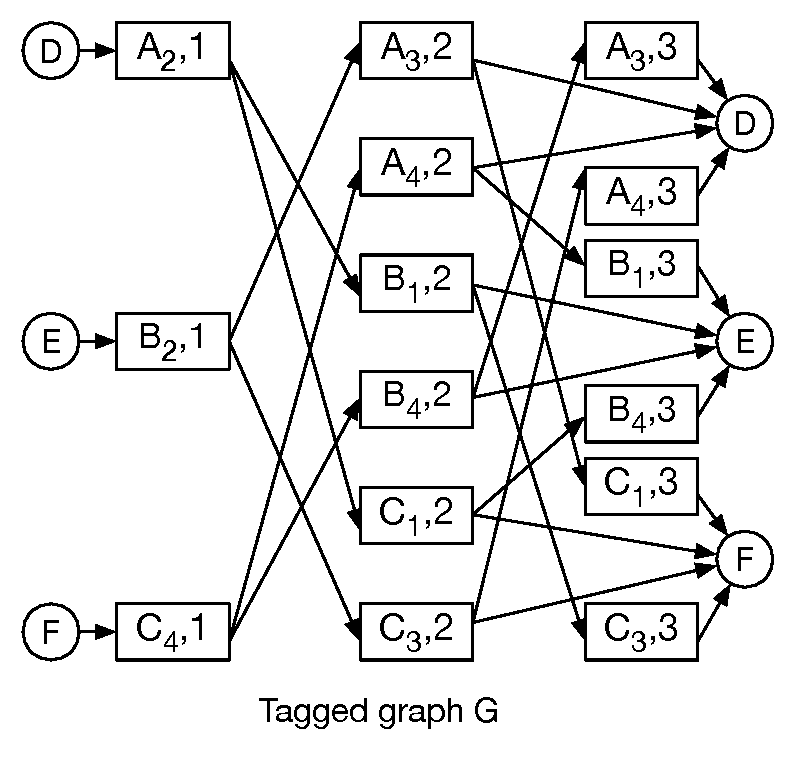
\includegraphics[width=0.4\textwidth] {figs/alo_walkthrough_b}
	}
	\caption{The input and output of Algorithm~\ref{alg:ttl}.}\label{fig:three_node}
\end{figure*}

As in \S\ref{sec:specific}, we will first design a tagging scheme that avoids
deadlock, then combine tags to reduce the number of required lossless queues.
For general graph without structure information, a straightforward tagging
system is to monotonically decrease the tag (thus, the priority) at every hop,
as described in Algorithm~\ref{alg:ttl}. 

\begin{algorithm}[t]
	\small
    \KwIn{Topology and expected lossless routes $R$}
	\KwOut{A tagged graph $G(V, E)$}
	$V \gets Set()$\;
	$E \gets Set()$\; 
	\For{each path $r$ in $R$} {
		$tag \gets 0$\;
		\For{each hop $h$ in $r$} {
			$V \gets V \cup \{(h, tag)\}$\;
			$E \gets E \cup \{lastHop\rightarrow(h, tag)\}$\;
			$tag \gets tag+1$\;
		}
	}
	\Return{$G(V, E)$}\;
    \caption{A brute-force tagging system that decreases the tag by one every hop.}
	\label{alg:ttl}
\end{algorithm}

It is easy to verify that the graph generated by this algorithm meets the two
requirements specified earlier, and thus it guarantees deadlock freedom.
Figure~\ref{fig:three_node} shows a small example, including the topology, the
set of desired lossless paths, the generated graph, and the corresponding rule
lists for each node.  

Of course, with just this basic algorithm, we may end up with too many tags
(i.e. lossless priorities) -- in fact, as many as diameter of the
network~\cite{xxx}. This is why we need 4 lossless priorities for the example in
Figure~\ref{fig:three_node}.  We now show how to combine tags to reduce the
number of lossless queues needed.

\subsection{Combining tags} 

The tags generated by Algorithm~\ref{alg:ttl} can be combined to reduce the
number of required lossless queues.  Algorithm~\ref{alg:greedy} uses a greedy
heuristic for this purpose.  It works by greedily combining as many nodes in
$G(V,E)$ as possible into each micropath subspaces under CBD-free constraint. To
ensure the monotonic property, we start from combing the nodes with largest tag
to smallest tag in the brute-force tagging system.  Obviously, the monotonic
property will still hold after combination. 

\begin{algorithm}[t]
	\small
    \KwIn{The brute-force tagged graph $G(V, E)$}
	\KwOut{A new tagged graph $G'(V', E')$ that has small $|\{G'_k\}|$}
	Initialize $V'$, $E'$, $V_{tmp}$, $E_{tmp}$ as empty $Set()$\;
	$t' \gets 0$\;
	\For{$t \gets 0$ \textbf{to} $maxTag$} {
		\For{each $(A_i, t)$ in $V$ whose tag is $t$} {
			$V_{tmp} \gets V_{tmp} \cup \{(A_i, t')\}$\;
			$E_{tmp} \gets E_{tmp} \cup \{$edges of $(A_i, t)$, change $t$ to $t'\}$\;
			\uIf{$G_{tmp}(V_{tmp}, E_{tmp})$ is acyclic} {
				$V' \gets V' \cup \{(A_i, t')\}$\;
				$E' \gets E' \cup \{$edges of $(A_i, t)$, change $t$ to $t'\}$\; 
			}
			\Else{
				$V' \gets V' \cup \{(A_i, t'+1)\}$\;
				$E' \gets E' \cup \{$edges of $(A_i, t)$, change $t$ to $t'+1\}$\;
				$V_{tmp} \gets V_{tmp} \backslash \{(A_i, t')\}$\;
				$E_{tmp} \gets E_{tmp} \backslash \{$edges of $(A_i, t')\}$\;
			}
		}
		\uIf{$V'$ contains nodes of tag $t'+1$} {
			$t' \gets t'+1$\;
			$V_{tmp} \gets \{$nodes in $V'$ with tag $t'+1\}$\;
			$E_{tmp} \gets \{$edges in $V'$, both ends have tag $t'+1\}$\;
		}
	}
	\Return{$G'(V', E')$}\;
    \caption{Greedily minimizing the number of micropath subspaces by merging brute-force tags.}
	\label{alg:greedy}
\end{algorithm}

\begin{figure}[t]
	%\vspace{-0.1in}
	\centering
	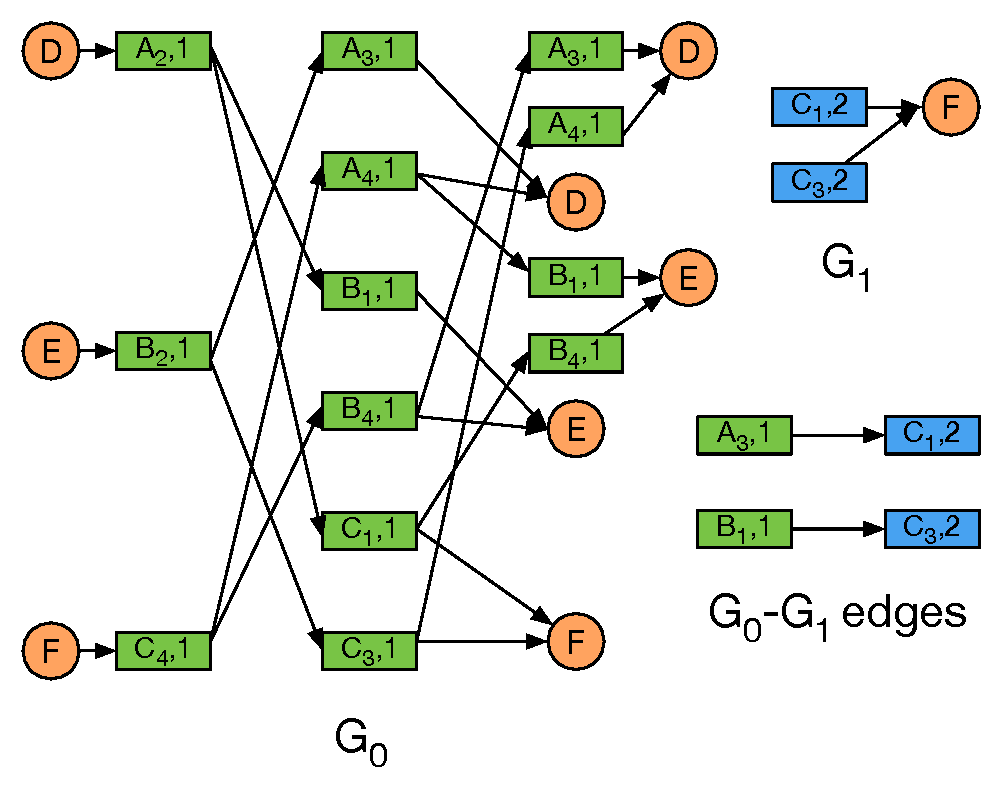
\includegraphics[width=0.48\textwidth] {figs/alo_walkthrough_c}
	\caption{Algorithm~\ref{alg:greedy} output for the example in Figure~\ref{fig:three_node}.}
	\label{fig:greedy}
\end{figure}

In  Figure~\ref{fig:greedy} we see Algorithm~\ref{alg:greedy} in action to
minimize the $G(V,E)$ from Figure~\ref{fig:three_node}. We see that the number
of tags is reduced to {\em two}.

\subsection {Discussion}
\label{subsec:caveats}

\para{Algorithm runtime:}. Algorithm~\ref{alg:greedy} is efficient. Given $maxTag$ 
(denoted as $T$ below), which equals to the longest path in {\em lossless routes} and
total number of switches $S$, $G(V,E)$ can have at most have $S \times T$ nodes.
Each node will be examined exactly once for checking whether $G_{tmp}$ is acyclic.
Checking whether $G_{tmp}$ is acyclic with a newly added node requires a Breadth-First Search,
with runtime complexity of $O(|V_{tmp}| + |E_{tmp}|)$. $|V_{tmp}|$ is bounded by the number
of switches $S$, and $|E_{tmp}|$ is bounded by the number of links, $L$, in the network.
Therefore, the total runtime complexity is $O(S \times T \times (S+L))$.

\para{Number of tags:} Algorithm~\ref{alg:greedy} significantly reduces the
number of tags on topology other than Clos. For example, it gives optimal
results for BCube topology without requiring any BCube-specific changes -- a
$k$-level BCube needs $k$ tags to prevent deadlock with default routing. The
results are promising even for unstructured topology like Jellyfish.  For
example, Jellyfish with 1000 nodes require only five tags with shortest-path
routing. See \S\ref{sec:eval} for details.

\begin{figure}[t]
	%\vspace{-0.1in}
	\centering
	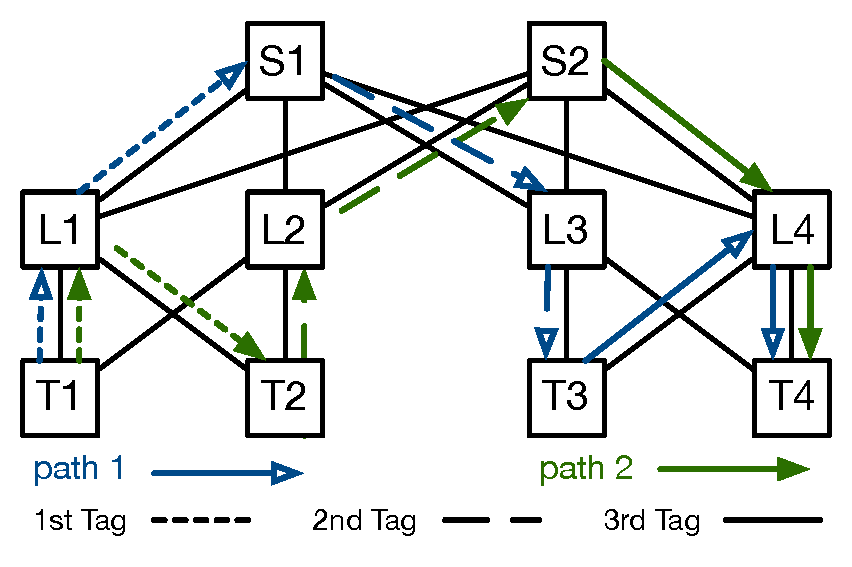
\includegraphics[width=0.48\textwidth] {figs/nonoptimal_example}
	\caption{Algorithm~\ref{alg:greedy} does not output optimal result for Clos with 1-bounce paths.}
	\label{fig:nonoptimal}
\end{figure}

\para{Optimality:}
Algorithm~\ref{alg:greedy} may not always return the optimal solution. For example, 
consider the simple three-layer Clos network in Figure~\ref{fig:nonoptimal}. 
Assuming ``normal'' and ``1-bounce'' paths must be lossless,  
we know the optimal tagging system only requires {\em two} lossless queues. However, the 
greedy algorithm will output {\em three} lossless queues. The reason is that 
Algorithm~\ref{alg:greedy} does not combine bounces that happen when the packet is going up
and when the packet is coming down. As a result, it has to 
assign a separate priority for each case, as shown in Figure~\ref{fig:nonoptimal}.
The fundamental reason is that generic algorithm does not fully utilize the inherently 
characteristics of structured topology like Clos. 

However, we do note that the number of tags in the solution of
Algorithm~\ref{alg:greedy} is an upper bound on the optimal solution.  Without
any assumptions, the worst case is the same as using the brute-force solution,
which require as many tags as the length of longest lossless route, $T$.
However, if we know that the smallest cycle in lossless routes is longer than
$l$, the output number of tags is bounded by $\lceil T/l \rceil$. We omit the
proof for brevity.

\para{Multiple application classes:} Sometimes, system administrators need to
use multiple lossless priorities to keep different traffic classes from impacting each
other. For example, in~\cite{dcqcn} congestion notification packets were
assigned a separate lossless class from data traffic to ensure that they would
not just be delivered losslessly, but also would not be held up behind data
traffic.

A n{\"a}ive way to use \sysname{} in such cases is to treat each application (or
traffic class) separately.  For example, in \S\ref{subsec:combine}, we showed
that for the Clos network, if we want to make  all paths with no more than $M$
bounces lossless, we need $M+1$ priorities. If there are $N$ applications, the
n{\"a}ive approach would use $N*(M+1)$ priorities.  However, the switches may
not have sufficient buffer to support this large number of lossless queues
(\S\ref{subsec:pfcheadroom}.

However, if we are willing to trade off some isolation, we can proceed as
follows.  We start the first lossless class with tag 1, and uses tag upto $M+1$.
The second lossless class starts with tag 2, and change tags in the same way as
the first class.  That is, whenever it has a bounce, the tag will increase by
one. The second lossless class uses tag from 2 to $M+2$. This goes on until the
$N'th$ lossless class. The total number of tags and lossless classes required is
$M + N$. The operator can further reduce the number of tags required by allowing
some application classes to tolerate fewer bounces than others.

We can prove that there is still no deadlock after such mix, by revisiting two
properties described in \S\ref{subsec:specific_deadlock_free}. First, there is
still no deadlock within each tag, because each tag is still a set of
``up-down'' routing. Second, the update of tags is still monotonical. We omit
formal proof for brevity. 

The reduced isolation may be quite acceptable, since only a small
fraction of packets experience one-bounce and may mix with traffic in the next
lossless class. 

This technique can be generalized for the output of Algorithm~\ref{alg:greedy}.
We omit details.

\para{The need to specify expected lossless paths:} The need to specify expected
lossless paths is not a problem in practice. For Clos networks, it is easy to
enumerate paths with any given limit on bouncing. For a general topology, as long
as the routing is traffic agnostic, it is usually easy to determine what routes
the routing algorithm will compute -- e.g. BGP will find shortest AS path etc.
In case an SDN controller is used, the controller algorithm can be used to
generate the paths under a variety of conditions. Even for traffic aware
routing, the operator can run a variety of simulations. 

The reader may also dislike the possibility that we eventually push a wayward
packet into a lossy queue. We stress that we do this only as a last resort, and
we reiterate that it does not mean that the packets are automatically or
immediately dropped. 
